\documentclass{article}
\usepackage{amsmath,amsfonts,color,amsthm,ifpdf}
\usepackage{algorithm,algorithmic}

\ifpdf
 \usepackage[pdftex]{graphicx}
\else
  \usepackage[dvips]{graphicx}
\fi

% Margins for plain pagestyle
\oddsidemargin=0.0in
\textwidth=6.5in
\textheight=9.0in
\topmargin=-0.5in



\title{Multigrid preconditioning for regularized least-squares problems}
\author{Matthias Bolten, Misha E. Kilmer, and Scott P. MacLachlan}

\begin{document}
\maketitle

\begin{abstract}
For many inverse problems, regularization is a key step in ensuring
fidelity of the recovered solution and overcoming noisy data or
uncertain forward models. For imaging problems, in particular,
classical regularization based on the L2 norm of the solution gradient
is well-known to be a poor choice, as it fails to preserve natural
edges in the recovered solution, and so minimization based on the L1
norm or total variation is generally preferred. In this talk, we
consider solution of the sequence of linear systems that arise when
such a regularized problem is solved using a reweighed least-squares
approach to resolve the regularization term. Particular attention is
paid to the selection of components of a multigrid preconditioner for
different ranges of the regularization parameter value.  {\bf Pasted
  from Copper Mountain abstract - needs more work!}
\end{abstract}


\section{Introduction}



In this paper, we are interested in designing efficient solvers for the sequence of least regularized least squares problems
\begin{equation}  \min_{x} \| K x - b \|_2^2 + \lambda^2 \| R^{(i)} x \|_2^2 \end{equation}
or equivalently
\[ \min_x \left\| \left[ \begin{matrix} K \\ \lambda R^{(i)} \end{matrix} \right] x - \left[ \begin{matrix} b \\ 0 \end{matrix} \right] \right\|_2 \]
or 
\[ (K^TK + \lambda^2 L^T (W^{(i)})^2 L ) x = K^T b \]
where 
\[ R^{(i)} = W^{(i)} L \] 
for $L$ the discrete gradient, and $W^{(i)}$ is a diagonal weighting, and we asume the ``best'' value of the regularization parameter for this $i$th problem, $\lambda^{(i)}_{*}$, is {\bf not} known a priori.   Such problems
frequently arise in situations where the weights would ideally be computed from the desired $x_{true}$, but as this is unknown the weights are recomputed adaptively from increasingly better estimates of the desired solution.    
In our numerical examples, we consider two types of weightings from recent literature:  one which is designed to give solutions with ``sparse'' gradients \cite{IRLS} and one which is designed to preserve edges \cite{KilmerEtalICIAM15}.  

We will consider only
one well-known heuristic for estimating $\lambda^{(i)}_*$ -- the L-curve criterion -- but our solvers would also be applicable in scenarios where other selection mechanisms are used.       
The L-curve \cite{OlearyHansen,etc} is a parametric plot of $( \log_10 \|K x_{\lambda} - b \|_2,\log_10 \| R^{(i)} x_{\lambda} \|_2)$ as a function of $\lambda$.   The general idea is that the point of maximum positive curvature occurs where there is a good balance between the effect of the regularization term and data-fidelity term.   (Forward reference to a plot in the paper).   

The obvious approach is to ``solve'' on of the equivalent forms of (\ref{eq:sequence}) for a few choices of $\lambda$ and then plot the curve.   If implemented naively, however, this is expensive because
   \begin{itemize}
      \item When $\lambda$ is small,   $\left[ \begin{matrix} K \\ \lambda R^{(i)} \end{matrix} \right] $ is likely to be ill-conditioned, as the emphasis is on the ill-conditioned top block.   Thus, many iterations are required for an {\it accurate} solution.
      \item When $\lambda$ is large, the emphasis is on the bottom block, but as $i$ increases, $R^{(i)}$ tends
      to be ill-conditioned due to more accurate diagonal weighting and near zero terms.
      \end{itemize}
      

Alternatively, hybrid iterative methods for the class of regularization operators we consider ($R^{(i)}$ rectangular with possible non-trivial null-space) we consider, in which $x$ is constrained to live in a k-dimensional subspace whose basis is generated by an iterative procedure for (\ref{eq:sequence}), have been proposed \cite{KilmerEspanolHansen,KilmerEtalICIAM15}.  Related methods, not immediately applicable for the case of non-rectangular $K$ and $L$ we consider here, are given in \cite{SilvaNagy15}.   Hybrid
methods have an advantage that, given a suitable $k$, the value of $\lambda_*^{(i)}$ can be chosen for the k-dimensional projected problem very cheaply, and only one subspace is needed/created for all values of $\lambda$.   The cost of the hybrid methods varies by algorithm, but matrix vector products with $K, R^{(i)}$ and their transposes are a necessary evil, and thus the minimum cost of any of these methods is $k$ times the sum of the costs for those products.   (MEK:  need to clean this up.  emphasize non-square A, L, means must use my appraoch, but and potential expense of our hybrid method and the fact other hybrids won't work unless you could transform to standard form, then you need A-weighted pseudoinverse which is very expensive per iteration.) 

Our goal in this paper is to modify the ``obvious'' approach so that it is provides a computationally viable algorithm.
Ingredients:
   \begin{itemize}
     \item AMG preconditioning when $\lambda$ is larger and favors the diffusion like term.   
     \item Non-exact solves with $\lambda$ small (possibly combined with preconditioner for $A^TA$?  ), just to know enough about the l-curve to find the corner
     \item Leveraging properites of the l-curves as functions of $i$ to prune $\lambda$
     \end{itemize} 

 In \cite{Gazzola_etal_2020}, an inner-outer iteration scheme is
 developed for the solution of \eqref{eq:sequence}, where the diagonal
 weighting matrix is updated at each outer iteration, and a hybrid
 method is used to find both the optimal regularization parameter,
 $\lambda$, and solution of the resulting least-squares problem.  This
 hybrid algorithm is based on joint bidiagonalization (cf.,
 \cite{Kilmer_Hanson_Espanol_2007}), projecting the large
 least-squares problem into a manageable subspace where $\lambda$ can
 be selected by standard approaches (e.g., the discrepancy principle
 or an L-curve criterion) and the minimizers of the projected problem
 can be readily computed directly.  However, each step of the hybrid
 iterative regularization requires two calls to another iterative
 routine to determine a projection, and therefore each step of the
 hybrid iterative regularization can be expensive.  Here, we consider
 the same outer iteration as \cite{Gazzola_etal_2020}, but we replace
 the single hybrid iterative routine with a new, two-pronged technique
 aimed at improving the overall efficiency of the edge-preserving
 algorithm.  First, we introduce an effective multigrid preconditioner
 for the solution of the global least-squares problem for fixed
 $\lambda$.  Secondly, we make use of the fact that we solve a
 sequence of least-squares problems for different values of $\lambda$
 to introduce improved initial guesses for the solution of each
 problem, improving the overall efficiency of the
 multigrid-preconditioned solves.  Finally, in this setting, we make
 use of an observed relationship between the optimal regularization
 parameters selected for each outer iteration to reduce the search
 space for regularization parameters within the inner iteration.


\section{Problem Formulation}
In this paper, we focus on an iterative approach to the solution of
ill-posed problems arising from the use of non-quadratic
regularization terms.  Consider the regularized system
\[
\min_x \|Kx-b\|^2 + \lambda^2 \mathcal{R}(x),
\]
where $\mathcal{R}(x)$ is some regularization term and $\lambda$ is
the regularization parameter, to be chosen using a standard L-curve
approach \cite{OlearyHansen,etc} or other means.  We specifically
consider the case where $\mathcal{R}(x) \approx \|Lx\|_\ast^2$, for
some norm (or weaker measure) applied to the discrete gradient of $x$.


\section{Outer Iteration}

We consider the solution of the regularized problem
\begin{equation}
\label{eq:regularized}
\min_{x} \|Kx-b\|^2 + \lambda^2\|WLx\|^2,
\end{equation}
where the equation $Kx=b$ represents a ``data'' term, where $b$ is
(noisy) data coming from some imaging process represented by $K$, and
the second term is a regularization term.  Here, $L$ is a discrete
gradient matrix, and $W$ is a diagonal weighting matrix with weights
in the range of $[0,1]$.  An equivalent formulation comes from first
writing this as a rectangular block least-squares problem,
\[
\min_{x} \left\| \left[\begin{array}{c} K \\ \lambda
      WL\end{array}\right]x - \left[\begin{array}{c} b \\ 0 \end{array}\right]\right\|^2,
\]
and, then, consider the resulting normal equations,
\begin{equation}
\label{eq:normal}
\left(K^TK + \lambda^2 L^TW^2L\right)x = K^Tb.
\end{equation}
Since $L$ is a discrete gradient, the second matrix in this expression
corresponds to a variable-coefficient diffusion operator (with
diffusion coefficient related to the weights in $W$), while the first
matrix and right-hand side come from the standard normal equations for
$Kx=b$.

Overall, this comes from a nonlinear problem, where we wish to choose
$x$, $W$, and $\lambda$ to minimize this functional while doing
something (iteration to drive $\ell_2$ regularization towards $\ell_1$
regularization).  We consider the case of fixed $W$, in the context of
this outer iteration.  At each step of the outer iteration, we need to
choose a good regularization parameter, $\lambda$, and find the
solution, $x$, for that value of $\lambda$.

Describe outer iteration for choosing $W$, so that $\|WLx\|_2 \approx
\|Lx\|_1$, then middle iteration for choosing $\lambda$ for fixed $W$,
and L-curve criteria, then need for an inner iteration to solve for
$x$ given $W$ and $\lambda$.


\section{Multigrid Algorithm}
Multigrid methods are optimal solvers for systems arising from the
discretization of elliptic PDEs. As noted before in \eqref{eq:normal}
the second matrix $L^T W^2 L$ corresponds to a variable-coefficient
diffusion operator on a two-dimensional grid. This can be treated
using multigrid. The variable coefficients that pose problems to
geometric multigrid methods can be treated using algebraic multigrid
that selects the coarse grid variables to treat this variability properly.

The first matrix in \eqref{eq:normal} corresponds to the operator that
has to be inverted. Usually, this is an integral operator, that is not
treated properly by algebraic multigrid. As the effective ratio
between the first and the second matrix in the system to be solved
depends on $\lambda$ we base our solver choice on the size of lambda
relative to the size of the singular values of $K^T K$ and $L^T W^2
L$.

For fixed $W$, the problem posed in \eqref{eq:regularized} is considered in 3 regimes:
\begin{enumerate}
\item When $\lambda > C \frac{\sigma(K)}{\sigma{WL}}$, where
  $\sigma(K)$ is the largest singular value of $K$ and $\sigma{WL}$ is
  the largest singular value of $WL$.  In this regime, the
  regularization (diffusive) term is dominant.
\item When $C \frac{\sigma(K)}{\sigma{WL}} > \lambda > c
  \frac{\sigma(K)}{\sigma{WL}}$, for $\mathcal{O}(1)$ constants $c$
  and $C$, the two terms in \eqref{eq:regularized} are {\it in
    balance}.
\item When $\lambda < c \frac{\sigma(K)}{\sigma{WL}}$, the data term
  in \eqref{eq:regularized} is dominant.
\end{enumerate}

In the first two cases, the diffusive term is significant, so the use
of a mulitigrid method is viable. We construct a multigrid method for
the regularized problem \eqref{eq:regularized} by reducing the size of
our solution, only. In terms of the block least-squares formulation
\eqref{eq:block-ls} the coarse grid correction corresponds to finding
a correction in the range of $P$ minimizing
\[
\min_{y_c}\left\| \left[\begin{array}{c} K \\ \lambda
      WL\end{array}\right](\hat{x}+Py_c) - \left[\begin{array}{c} b \\ 0 \end{array}\right]\right\|^2.
\]
Due to the equivalence of the least-squares problem and the solution
of the normal equations \eqref{eq:normal} the coarse-grid solution $y_c$ is then characterized as the solution to
\[
\left(P^TK^TKP + \lambda^2P^TL^TW^2LP\right)y_c =
P^T\left[\begin{array}{c} K \\ \lambda WL\end{array}\right]^T
\left(\left[\begin{array}{c} b \\ 0 \end{array}\right] - \left[\begin{array}{c} K \\ \lambda
      WL\end{array}\right]\hat{x}\right),
\]
where the right-hand side is the restriction of the residual in the
normal equations associated with $\hat{x}$.

The equivalence of the formulations allows to design a multigrid
algorithms for the normal equations \eqref{eq:normal}, and apply it
directly to the sparse matrices in \eqref{eq:regularized}. As $K^TK$
can get dense, this results in a tremendous reduction of compute time,
further efficient implementations of the application of $K$, e.g.,
using fast transformations, can be used directly.

To obtain $P$, only the matrix $A = L^T W^2 L$ is considered. We apply a
standard AMG setup phase to $A$ to create a hierarchy of interpolation
operators, $P$, and coarse-grid operators, $A_c = P^TAP$ (using
Galerkin coarsening).  From these interpolation operators, we also
create the \textit{one-sided} coarse-grid operators $K_c = KP$ and $(WL)_c =
WLP$, at all levels in the multigrid hierarchy. All that remains is to
specify the multigrid relaxation scheme and cycling parameters.  In
all that follows, we consider only multigrid V-cycles, as W-cycles (or
F-cycles) do not appear to be beneficial.

In the diffusion-dominated regime, the solution of
\eqref{eq:regularized} is primarily determined by the diffusive term
and, as such, we propose a multigrid smoother that is appropriate for
this term.  While classical AMG applied to \eqref{eq:normal} would
typically use a Gauss-Seidel relaxation scheme, this is not
appropriate here, since it would require knowledge of the (dense)
lower-triangular part of $K^TK$.  Instead, we use a red-black-ordered
Jacobi iteration, which allows us to make use of efficient
matrix-vector products with $K$ and $WL$ and their transposes.
Following reduction-based multigrid ideas \cite{}, we use only a
single sweep of pre-relaxation, in a CF ordering, first computing
updates to the coarse-grid points, then to those points on the fine
grid that are not directly represented on the coarse grid.  For each
of these sub-sweeps, we compute a full residual of the rectangular
form of the system,
\[
\hat{r} = \left[\begin{array}{c} b \\ 0 \end{array}\right] -
\left[\begin{array}{c} K \\ \lambda WL\end{array}\right]\hat{x}
\]
but then compute a Jacobi-like update at only the points, $j$, under
consideration, as
\[
\hat{x}_j + {\left(\left[\begin{array}{cc} K^T & \lambda
      L^TW\end{array}\right]\hat{r}\right)_j}/{ \left(K^TK +
  \lambda^2L^TW^2L\right)_{jj}}.
\]
We note that this requires computing only part of the matrix-vector
product with $\left[\begin{array}{cc} K^T & \lambda
    L^TW\end{array}\right]$ and the diagonal entries of $K^TK +
\lambda^2L^TW^2L$.  With this approach, a CF sweep of relaxation costs
the same as 3/2 matrix-vector products with the normal equations (when
done implicitly using the sparse matrices $K$ and $WL$).

Numerical experiments below show that this is an efficient relaxation
scheme for the problem, leading to good multigrid convergence, only
for sufficiently large $\lambda$.  In the second case, when the two
terms are more in balance, the multigrid approach can still be
effective, but the CF relaxation scheme is no longer appropriate,
since the diffusion term is not dominant.  Here, to better reflect the
impact of $K$ on the linear system, we use the CG algorithm as a
relaxation scheme, taking five steps of CG on the normal equations
(with no preconditioner).  Probably need some references here about
using CG as a smoother - Wim's papers on Helmholtz + GMRES, Randy Bank
paper, Xuejun Xu cascadic MG paper???...

We note that the interpolation and coarse-grid operators used above do
not depend on $\lambda$ and, thus, can be formed once for each choice
of $W$ and reused for all values of $\lambda$ for which a multigrid
iteration is needed.

When $\lambda$ is small compared to $\frac{\sigma(K)}{\sigma(WL)}$,
then the problem is essentially equivalent to the unregularized
problem $min_x \|Kx-b\|^2$.  In this case, ... Here, we rely on the
fact that the outer (nonlinear) iteration is aiming to choose $W$ so
that the two terms are in balance.  Thus, while it is important to get
a sufficiently accurate solution when $\lambda$ is small to drive the
nonlinear iteration, we are not concerned with getting high levels of
accuracy in this case (since it occurs only early in the outer
(nonlinear) iteration).  In this case, there is little expected
benefit from a coarse-grid correction based on the diffusive term, so
we consider only a simple iteration.  We use unpreconditioned CG on
the normal equations, allowing up to 50 steps.  In practice, this
yields relatively little improvement on using the solution from the
next-largest $\lambda$ value as the initial guess, and the improvement
to be gained decreases as $\lambda$ does.

{\bf Ask Misha if there's something more reasonable to be done in the
  case of smallest values of $\lambda$.}



\section{Numerical Results}
% !TEX root = regularized.tex
The described methods have been implemented and tested using MATLAB R2020a and the toolboxes AIR Tools II \cite{art:HANS18} and IR Tools \cite{art:GAZZ19}. We stop the outer iteration when
\[
\|L x^{(\ell)}\|_2^2 < \|L x^{(\ell-1)}\|_2^2,
\]
as proposed in \cite{Gazzola_etal_2020}. The multigrid preconditioned
FGMRES iteration was used (without restarting), with a stopping
criterion of a reduction of the $\ell^2$ norm of the residual of the normal equations to below $10^{-6}$. As possible values for the regularization parameter, $\lambda$, in the outer iteration, we used 30 values equally distributed on a logarithmic scale between $10^{-3}$ and $10^{2}$ using MATLAB's \texttt{logspace(2,-3,30)} command.

\subsection{Usage of the solution of the previous iteration}
Before evaluating the proposed method in detail, we want to highlight the effect of using the solution of the previous outer (and inner) iteration at each step. Instead of choosing a zero initial guess, as would be commonly used, we use the best available approximation to the solution as the initial guess for each linear solve.  For the first inner iteration with each outer iteration, this is the solution of the previous outer iteration.  For each subsequent inner iteraiton, it is the solution of the previous inner iteration.  We use a tomography example, using the Shepp Logan phantom of different sizes with different amounts of added noise, created using IR Tools' \cite{art:GAZZ19} \texttt{PRtomo} and \texttt{PRnoise} routines. The resulting average number of inner iterations per outer iteration is plotted in Fig.~\ref{fig:zero_initial_guess_vs_previous_iteration}, demonstrating that, in general, using the available information reduces the number of inner iterations needed.  Thus, in all further experiments we use these improved initial guesses.
\begin{figure}[htbp]
\begin{center}
\includegraphics{figures/zero_initial_guess_vs_previous_iteration}
\caption{Number of inner iterations needed in each outer iteration of the method applied to the Shepp Logan phantom. Solid lines represent the average number of iterations needed when using a zero initial guess, and dashed lines represent the same number when using the solution of the previous inner (or outer) iteration.}
\label{fig:zero_initial_guess_vs_previous_iteration}
\end{center}
\end{figure}

\subsection{Effect of pre- and post-relaxation}
\label{ssec:relaxation_comparison}
An important parameter that has to be chosen in multigrid methods is the number of pre- and post-relaxation steps. To be able to do this, we study the dependence of the convergence rate on the number of pre- and post-relaxation steps. For that purpose, we study the same tomography example as before, limiting ourselves to size $128 \times 128$ with 1\% added noise. We tested V(0,1)-, V(1,1)-, V(1,2)-, V(2,1)- and V(2,2)-cycles for this problem. For each outer iteration, we recorded the minimal, maximal and average number of inner iterations needed for the different values of $\lambda$ that were evaluated in the respective outer iteration. The resulting maximal, minimal and average numbers of iterations is depicted in Fig.~\ref{fig:its_cycling}, while the average number of iterations needed in each outer iteration can also be found in Table~\ref{tab:its_cycling}. As can be seen from these results, the difference in performance between V(2,1) cycles and V(2,2) cycles is small, and the former even perform better for some early outer iterations.  On the other hand, particularly for early outer iterations, the improvement given by using V(2,1) cycles over V(1,1) or V(1,2) cycles is clear.   Therefore, we use V(2,1) cycles in the rest of our numerical experiments.
\begin{figure}[htbp]
\begin{center}
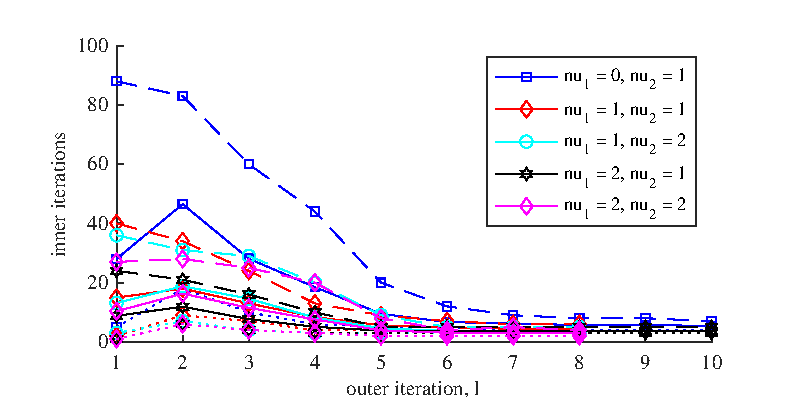
\includegraphics{figures/its_cycling}
\caption{Number of inner iterations needed in each outer iteration of the method applied to the Shepp Logan phantom of size $128 \times 128$ with 1\% noise for different multigrid cycles. Solid lines represent the average number of iterations needed for the different values of lambda, dashed lines the maximum number of iterations, and dotted lines the minimum.}
\label{fig:its_cycling}
\end{center}
\end{figure}
\begin{table}[htp]
\caption{Average number of inner iterations needed in each outer iterations of the method applied to the Shepp Logan phantom of size $128 \times 128$ with 1\% noise for different multigrid cycles.}
\begin{center}
\begin{tabular}{|l|r|r|r|r|r|r|r|r|r|r|}
\hline
& \multicolumn{1}{c|}{1} & \multicolumn{1}{c|}{2} & \multicolumn{1}{c|}{3} & \multicolumn{1}{c|}{4} & \multicolumn{1}{c|}{5} & \multicolumn{1}{c|}{6} & \multicolumn{1}{c|}{7} & \multicolumn{1}{c|}{8} & \multicolumn{1}{c|}{9} & \multicolumn{1}{c|}{10} \\
\hline
V(0,1) & 28.0 & 46.5 & 28.1 & 18.5 & 9.5 & 6.7 & 6.2 & 5.7 & 5.7 & 5.4 \\
V(1,1) & 15.0 & 18.0 & 13.0 & 8.4 & 5.6 & 5.0 & 4.4 & 4.2 & \multicolumn{1}{c|}{---} & \multicolumn{1}{c|}{---}\\
V(1,2) & 13.1 & 18.8 & 14.6 & 8.2 & 4.6 & 3.7 & 3.5 & 3.4 & \multicolumn{1}{c|}{---} & \multicolumn{1}{c|}{---} \\
V(2,1) & 8.8 & 11.9 & 7.7 & 5.1 & 3.8 & 3.8 & 3.7 & 3.7 & 3.6 & 3.6 \\
V(2,2) & 10.4 &16.3 & 11.5 & 7.6 & 3.9 & 3.1 & 3.0 & 2.9 & \multicolumn{1}{c|}{---} & \multicolumn{1}{c|}{---} \\
\hline
\end{tabular}
\end{center}
\label{tab:its_cycling}
\end{table}%


\subsection{Effect of trimming the L-curve}
\label{ssec:trimming_numerical}
Using the V(2,1)-cycle and 1\% noise, we next consider the effect of the proposed trimming of the L-curve for a computer tomography example using the Shepp Logan phantom of sizes $64 \times 64$, $128 \times 128$ and $256 \times 256$. We compare the L-curve algorithm from \cite{OlearyHansen} applied to the whole range of values of $\lambda$ with two variants that apply it to a smaller range of values. The first variant uses only the smallest 10 values of $\lambda$ when computing the solution to the first outer iteration and, after that, takes the range described above with the seven larger values of $\lambda$ than the optimal value chosen at the previous outer iteration, that value itself, and the two immediately smaller values. The second variant uses the whole range of $\lambda$ values at the first outer iteration but, from the second iteration onwards, follows the same strategy as the first variant. The regularization parameters chosen are depicted in Fig.~\ref{fig:shepp_logan_reg_params_with_and_without_trimming}. Here, we see that, for these examples, the first variant tends to choose a too small regularization parameter in the first iteration, leading to a larger number of iterations. The second variant, in contrast, choses almost exactly the same regularization parameters and shows the same algorithmic behavior as the variant without trimming, but at a little more than one third of the computational cost.
\begin{figure}[htbp]
\begin{center}
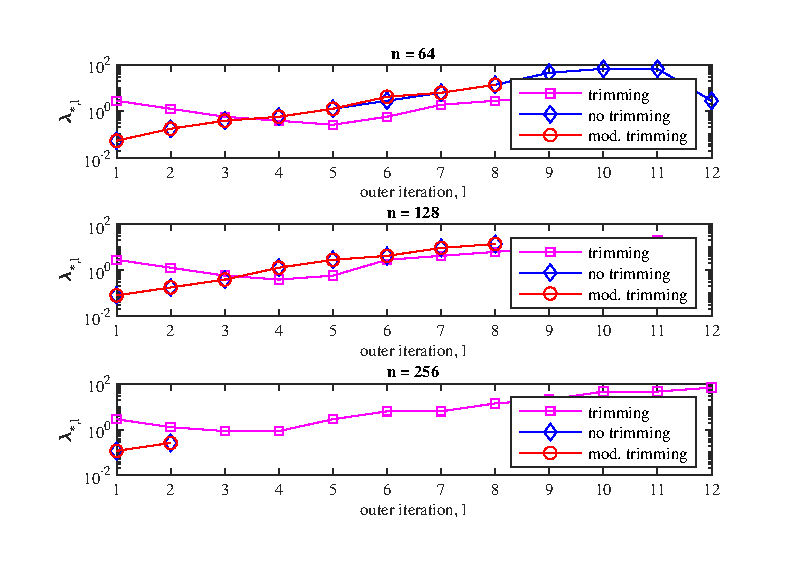
\includegraphics{figures/shepp_logan_reg_params_with_and_without_trimming}
\caption{Effect of trimming the L-curve for a full angle computer tomography using the Shepp Logan phantom with 1\% noise. Depicted are the regularization parameters chosen by the algorithm. The modified trimming uses trimming only after the first iteration.}
\label{fig:shepp_logan_reg_params_with_and_without_trimming}
\end{center}
\end{figure}

\subsection{Full angle computer tomography}
For the computer tomography example using the Shepp Logan phantom of sizes $64 \times 64$, $128 \times 128$ and $256 \times 256$, we now compare the performance of the algorithm for different noise levels. We used the modified trimming approach and a V(2,1)-cycle for preconditioning FGMRES for 0.5\% noise, 1\% noise, and 2\% noise. The resulting errors and the chosen regularization parameters can be found in Fig.~\ref{fig:shepp_logan_errs_and_reg_params} and in Table~\ref{tab:shepp_logan_errs_and_reg_params}. The minimal, maximal and average inner interations needed can be found in Fig~\ref{fig:shepp_logan_inner_its}. The initial and final reconstructions are in Fig.~\ref{fig:shepp_logan_initial_and_final}.

\begin{figure}[htbp]
\begin{center}
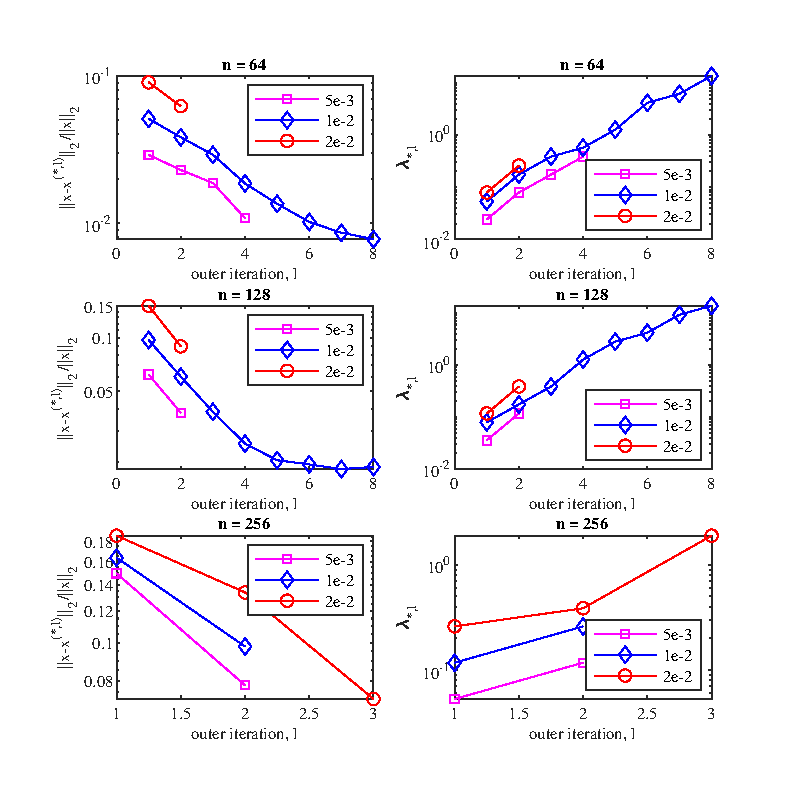
\includegraphics{figures/shepp_logan_errs_and_reg_params}
\caption{Errors (left) and regularization parameters chosen (right) for full angle computer tomography of the Shepp Logan phantom for different image sizes (by row) and noise levels.}
\label{fig:shepp_logan_errs_and_reg_params}
\end{center}
\end{figure}
\begin{table}[htp]
\caption{Errors and regularization parameters chosen for the Shepp Logan computer tomography example for different image sizes and 0.5\% noise.}
\begin{center}
\begin{tabular}{|r|r|r|r|r|r|r|r|r|r|r|}
\hline
\multicolumn{1}{|c|}{outer} & \multicolumn{2}{c|}{$n = 64$} & \multicolumn{2}{c|}{$n = 128$} & \multicolumn{2}{c|}{$n = 256$} \\\cline{2-7}
\multicolumn{1}{|c|}{iter.} & \multicolumn{1}{c|}{$\lambda$} & \multicolumn{1}{c|}{$\frac{\|x - x^{(*,\ell)}\|_2}{\|x\|_2}$} & \multicolumn{1}{c|}{$\lambda$} & \multicolumn{1}{c|}{$\frac{\|x - x^{(*,\ell)}\|_2}{\|x\|_2}$}  & \multicolumn{1}{c|}{$\lambda$} & \multicolumn{1}{c|}{$\frac{\|x - x^{(*,\ell)}\|_2}{\|x\|_2}$} \\
\hline
1 & 0.0291 & 0.0240 & 0.0621 & 0.0356 & 0.1495 & 0.1495 \\
2 & 0.0230 & 0.0788 & 0.0379 & 0.1172 & 0.0780 & 0.0780 \\
3 & 0.0187 & 0.1743 & -- & -- & -- & -- \\
4 & 0.0108 & 0.3857 & -- & -- & -- & -- \\
\hline
\end{tabular}
\end{center}
\label{tab:shepp_logan_errs_and_reg_params}
\end{table}%
\begin{figure}[htbp]
\begin{center}
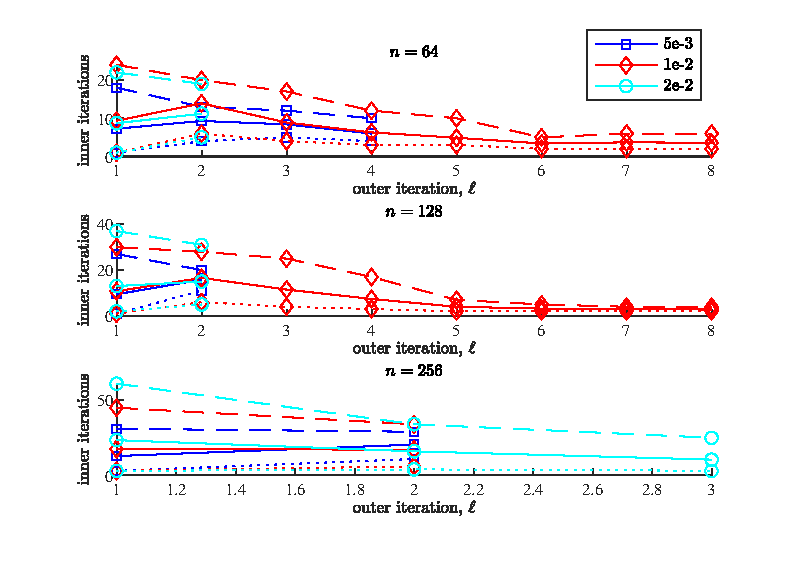
\includegraphics{figures/shepp_logan_inner_its}
\caption{Inner iterations for full angle computer tomography of the Shepp Logan phantom.  Solid lines represent the average number of iterations needed for the different values of lambda, dashed lines the maximum number of iterations, and dotted lines the minimum.}
\label{fig:shepp_logan_inner_its}
\end{center}
\end{figure}%
\begin{figure}[htbp]
\begin{center}
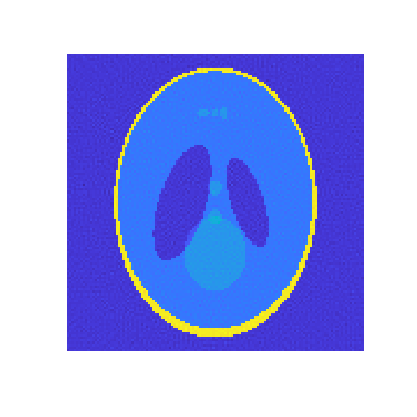
\includegraphics{figures/shepp_logan_initial}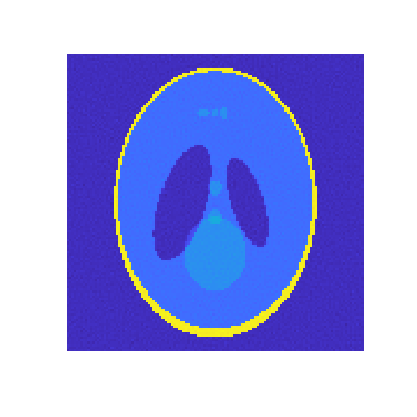
\includegraphics{figures/shepp_logan_final}
\caption{Initial and final image obtained for the Shepp Logan computer tomography example for size $128 \times 128$ and 0.5\% noise.}
\label{fig:shepp_logan_initial_and_final}
\end{center}
\end{figure}%

\subsection{Limited angle computer tomography}
We now consider a similar example for \textit{limited angle} computer tomography, using the grains example from IR tools \cite{art:GAZZ19}. We use the command \texttt{PRset('angles', 0:2:130, 'phantomImage', 'grains')} to set up the problem and choose sizes $64 \times 64$, $128 \times 128$, and $256 \times 256$. As before, we compare the performance using the modified trimming and a V(2,1)-cycle for preconditioning FGMRES with 0.5\% noise, 1\% noise, and 2\% noise. Fig.~\ref{fig:limited_angle_grains_errs_and_reg_params} and Table~\ref{tab:limited_angle_grains_errs_and_reg_params} show the resulting errors and the chosen regularization parameters. The initial and final reconstructions are in Fig.~\ref{fig:limited_angle_grains_initial_and_final}.
\begin{figure}[htbp]
\begin{center}
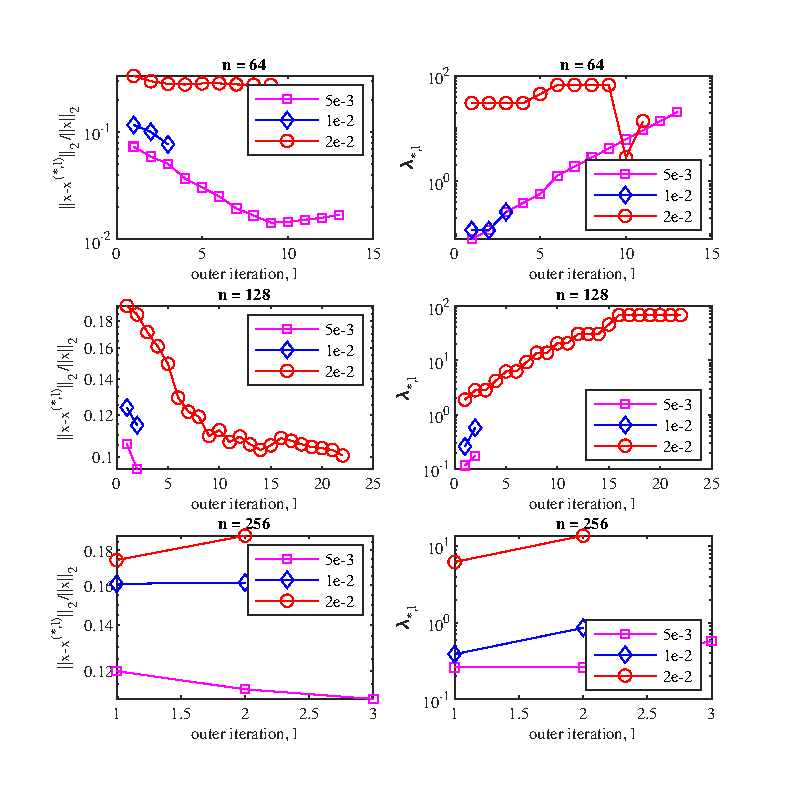
\includegraphics{figures/limited_angle_grains_errs_and_reg_params}
\caption{Errors (left) and regularization parameters chosen (right) for the 130-degree limited angle computer tomography of the grains example for different image sizes (by row) and noise levels.}
\label{fig:limited_angle_grains_errs_and_reg_params}
\end{center}
\end{figure}
\begin{table}[htp]
\caption{Errors and regularization parameters chosen for the 130-degree limited angle computer tomography of the grains example for different image sizes and 0.5\% noise.}
\begin{center}
\begin{tabular}{|r|r|r|r|r|r|r|r|r|r|r|}
\hline
\multicolumn{1}{|c|}{outer} & \multicolumn{2}{c|}{$n = 64$} & \multicolumn{2}{c|}{$n = 128$} & \multicolumn{2}{c|}{$n = 256$} \\\cline{2-7}
\multicolumn{1}{|c|}{iter.} & \multicolumn{1}{c|}{$\lambda$} & \multicolumn{1}{c|}{$\frac{\|x - x^{(*,\ell)}\|_2}{\|x\|_2}$} & \multicolumn{1}{c|}{$\lambda$} & \multicolumn{1}{c|}{$\frac{\|x - x^{(*,\ell)}\|_2}{\|x\|_2}$}  & \multicolumn{1}{c|}{$\lambda$} & \multicolumn{1}{c|}{$\frac{\|x - x^{(*,\ell)}\|_2}{\|x\|_2}$} \\
\hline
1 & 0.0734 & 0.0788 & 0.1057 & 0.1172 & 0.1199 & 0.1199 \\
2 & 0.0593 & 0.1172 & 0.0948 & 0.1743 & 0.1128 & 0.1128 \\
3 & 0.0507 & 0.2593 & -- & -- & 0.1092 & 0.1092 \\
4 & 0.0370 & 0.3857 & -- & -- & -- & -- \\
5 & 0.0305 & 0.5736 & -- & -- & -- & -- \\
6 & 0.0251 & 1.2690 & -- & -- & -- & -- \\
7 & 0.0194 & 1.8874 & -- & -- & -- & -- \\
8 & 0.0167 & 2.8072 & -- & -- & -- & -- \\
9 & 0.0143 & 4.1753 & -- & -- & -- & -- \\
10 & 0.0145 & 6.2102 & -- & -- & -- & -- \\
11 & 0.0152 & 9.2367 & -- & -- & -- & -- \\
12 & 0.0158 & 13.7382 & -- & -- & -- & -- \\
13 & 0.0169 & 20.4336 & -- & -- & -- & -- \\\hline
\end{tabular}
\end{center}
\label{tab:limited_angle_grains_errs_and_reg_params}
\end{table}%
\begin{figure}[htbp]
\begin{center}
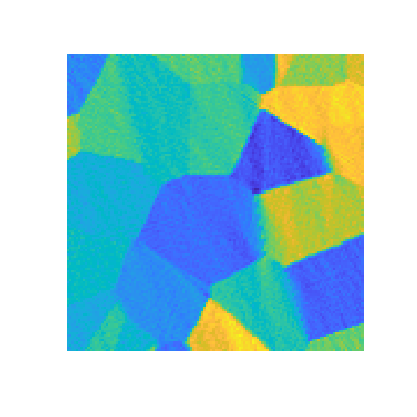
\includegraphics{figures/limited_angle_grains_initial}
\includegraphics{figures/limited_angle_grains_final}
\caption{Initial and final image obtained for the 130-degree limited angle computer tomography of the grains example for size $128 \times 128$ and 0.5\% noise.}
\label{fig:limited_angle_grains_initial_and_final}
\end{center}
\end{figure}

\subsection{Image deblurring}
To demonstrate that the methodology also works for other inverse problems, we now blur the grains example images of sizes $64 \times 64$, $128 \times 128$ and $256 \times 256$, using a discretized integral kernel for the $m \times n$ image represented by the Toeplitz matrix created using:
\begin{verbatim}

band1 = 8; sigma1=1.5*n/64; 
band2 = 7; sigma2=1.25*n/64;
z1 = [exp(-((0:band1-1).^2)/(2*sigma1^2)),zeros(1,n-band1)];
z1 = z1./(2*sum(z1)-1); z1=z1';
z2 = [exp(-((0:band2-1).^2)/(2*sigma2^2)),zeros(1,m-band2)];
z2 = z2./(2*sum(z2)-1); z2=z2';
A1 = toeplitz(z1); A1 = sparse(A1); 
A2 = toeplitz(z2); A2 = sparse(A2);
A = kron(A1,A2);

\end{verbatim}
As before, 0.5\%, 1\%, and 2\% noise are added to the blurred image and the method is applied using the same settings. The behavior of the algorithm is similar to the other cases and errors as well as regularization parameters are to be found in Fig,~\ref{fig:grains_blurring_errs_and_reg_params} and in Table~\ref{tab:grains_blurring_errs_and_reg_params}. The initial and final reconstruction are in Fig.~\ref{fig:grains_blurring_initial_and_final}.
\begin{figure}[htbp]
\begin{center}
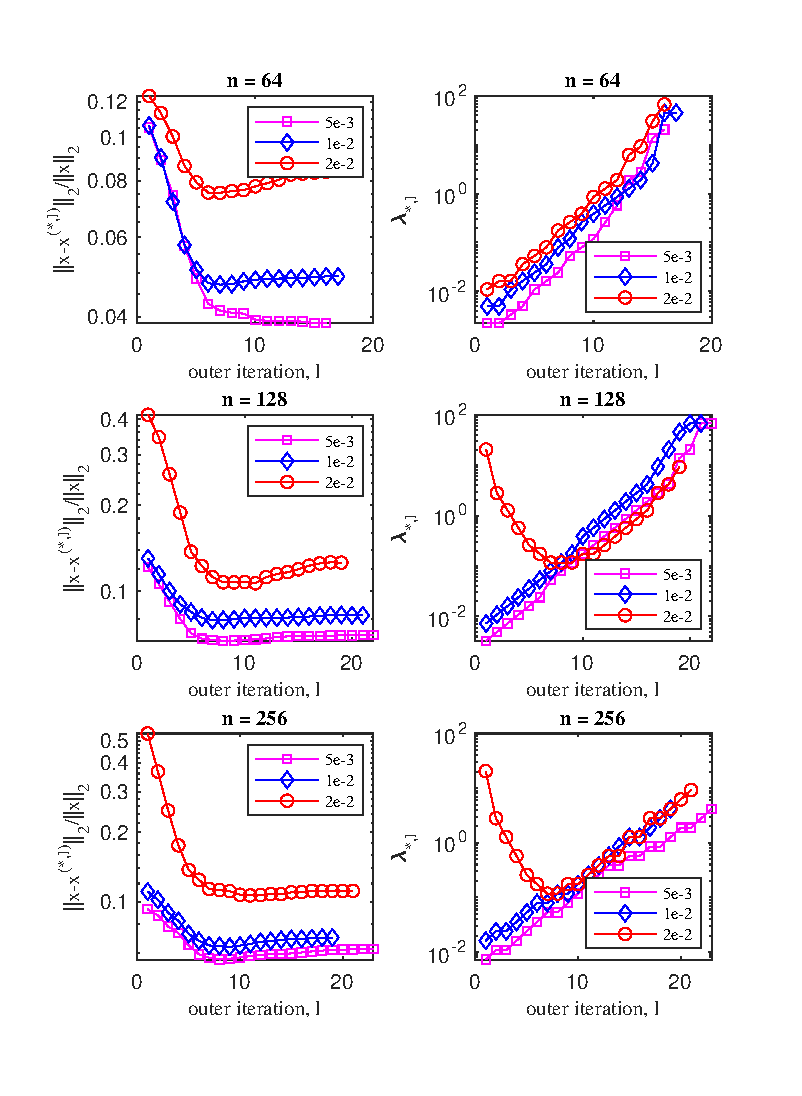
\includegraphics{figures/grains_blurring_errs_and_reg_params}
\caption{Errors (left) and regularization parameters chosen (right) for the blurred grains example for different image sizes (by row) and noise levels.}
\label{fig:grains_blurring_errs_and_reg_params}
\end{center}
\end{figure}
\begin{table}[htp]
\caption{Errors and regularization parameters chosen for the blurred grains example for different image sizes and 0.5\% noise.}
\begin{center}
\begin{tabular}{|r|r|r|r|r|r|r|r|r|r|r|}
\hline
\multicolumn{1}{|c|}{outer} & \multicolumn{2}{c|}{$n = 64$} & \multicolumn{2}{c|}{$n = 128$} & \multicolumn{2}{c|}{$n = 256$} \\\cline{2-7}
\multicolumn{1}{|c|}{iter.} & \multicolumn{1}{c|}{$\lambda$} & \multicolumn{1}{c|}{$\frac{\|x - x^{(*,\ell)}\|_2}{\|x\|_2}$} & \multicolumn{1}{c|}{$\lambda$} & \multicolumn{1}{c|}{$\frac{\|x - x^{(*,\ell)}\|_2}{\|x\|_2}$}  & \multicolumn{1}{c|}{$\lambda$} & \multicolumn{1}{c|}{$\frac{\|x - x^{(*,\ell)}\|_2}{\|x\|_2}$} \\
\hline
1 & 0.1051 & 0.0022 & 0.1215 & 0.0033 & 0.0928 & 0.0928 \\
2 & 0.0891 & 0.0022 & 0.1060 & 0.0049 & 0.0872 & 0.0872 \\
3 & 0.0746 & 0.0033 & 0.0920 & 0.0073 & 0.0781 & 0.0781 \\
4 & 0.0575 & 0.0049 & 0.0800 & 0.0108 & 0.0731 & 0.0731 \\
5 & 0.0486 & 0.0108 & 0.0715 & 0.0161 & 0.0648 & 0.0648 \\
6 & 0.0427 & 0.0161 & 0.0684 & 0.0240 & 0.0591 & 0.0591 \\
7 & 0.0413 & 0.0240 & 0.0677 & 0.0530 & 0.0571 & 0.0571 \\
8 & 0.0408 & 0.0530 & 0.0672 & 0.0788 & 0.0561 & 0.0561 \\
9 & 0.0406 & 0.0788 & 0.0673 & 0.1172 & 0.0566 & 0.0566 \\
10 & 0.0394 & 0.1172 & 0.0676 & 0.1743 & 0.0574 & 0.0574 \\
11 & 0.0392 & 0.2593 & 0.0680 & 0.2593 & 0.0581 & 0.0581 \\
12 & 0.0392 & 0.5736 & 0.0685 & 0.3857 & 0.0588 & 0.0588 \\
13 & 0.0391 & 1.8874 & 0.0693 & 0.5736 & 0.0592 & 0.0592 \\
14 & 0.0390 & 2.8072 & 0.0696 & 0.8532 & 0.0592 & 0.0592 \\
15 & 0.0387 & 13.7382 & 0.0698 & 1.2690 & 0.0597 & 0.0597 \\
16 & 0.0388 & 20.4336 & 0.0699 & 1.8874 & 0.0602 & 0.0602 \\
17 & -- & -- & 0.0700 & 2.8072 & 0.0609 & 0.0609 \\
18 & -- & -- & 0.0701 & 4.1753 & 0.0614 & 0.0614 \\
19 & -- & -- & 0.0702 & 13.7382 & 0.0619 & 0.0619 \\
20 & -- & -- & 0.0702 & 20.4336 & 0.0620 & 0.0620 \\
21 & -- & -- & 0.0703 & 67.2336 & 0.0622 & 0.0622 \\
22 & -- & -- & 0.0703 & 67.2336 & 0.0624 & 0.0624 \\
23 & -- & -- & -- & -- & 0.0625 & 0.0625 \\
\hline
\end{tabular}
\end{center}
\label{tab:grains_blurring_errs_and_reg_params}
\end{table}%
\begin{figure}[htbp]
\begin{center}
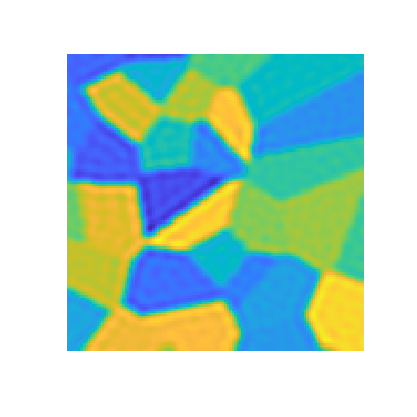
\includegraphics{figures/grains_blurring_initial}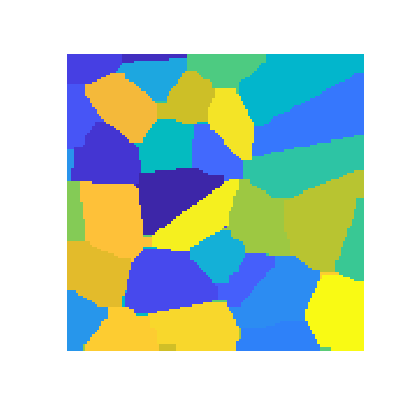
\includegraphics{figures/grains_blurring_final}
\caption{Initial and final image obtained for the blurred grains example for size $128 \times 128$ and 0.5\% noise.}
\label{fig:grains_blurring_initial_and_final}
\end{center}
\end{figure}

%As a first example we consider the Shepp-Logan phantom, generated by
%the MATLAB command \texttt{phantom}. We consider a version of size
%$64^2$ with added noise of level $0.5\%$, $1\%$ and $2\%$. The
%iteration was stopped, when the regularization error of the current
%solution $x^{(k)}$, measured as the 2-norm of $L^TW^2L$ applied to it,
%grew again, i.e., when
%\[
%  \| L^TW^2L x^{(k)} \|_2 > \| L^TW^2L x^{(k-1)} \|_2.
%\]
%In this case, the previous solution $x^{(k-1)}$ usually provides a
%good reconstruction.
%
%First, we ran the proposed algorithm for a full-angle Radon transform
%with 30 fixed values of $\lambda$, logarithmically spaced between
%$10^{-3}$ and $10^2$. The $\lambda$ chosen in each iteration can be
%found in Table~\ref{tab:chosen_lambda_all_lambda_full_angle}.
%
%\begin{table}
%  \begin{center}
%    \begin{tabular}{c|ccc|ccc}
%      Problem & \multicolumn{3}{|c}{full angle case} &
%                                                       \multicolumn{3}{|c}{limited
%                                                       angle case} \\
%      Noise & $0.5\%$ & $1\%$ & $2\%$ & $0.5\%$ & $1\%$ & $2\%$ \\
%      \hline
%      Iteration 1 & 0.0161 & 0.0356 & 0.0530 & 0.0161 & 0.0356 & 0.0530 \\
%      Iteration 2 & 0.0240 & 0.0530 & 0.0788 & 0.0240 & 0.0356 & 0.0788 \\
%      Iteration 3 & 0.0530 & 0.1172 & 0.2593 & 0.0356 & 0.0788 & 0.1172 \\
%      Iteration 4 & 0.0788 & 0.1743 & 0.3857 & 0.0530 & 0.1172 & 0.1743 \\
%      Iteration 5 & 0.1743 & 0.3857 & 0.8532 & 0.0788 & 0.1172 & 0.5736 \\
%      Iteration 6 & 0.3857 & 1.2690 & 1.2690 & 0.0788 & 0.1743 & 0.8532 \\
%      Iteration 7 & 1.2690 & 1.8874 & 2.8072 & 0.1172 & 0.2593 & 1.2690 \\
%      Iteration 8 & 2.8072 & 2.8072 & 6.2102 & 0.1172 & 0.5736 & 1.8874 \\
%      Iteration 9 & 6.2102 & 6.2102 & 9.2367 & 0.1743 & 0.8532 & 2.8072 \\
%      Iteration 10 & 13.7382 & 13.7382 & 13.7382 & 0.2593 & 1.2690 & 6.2102 \\
%      Iteration 11 & 30.3920 & 20.4336 & 30.3920 & 0.3857 & 1.8874 & 6.2102 \\
%      Iteration 12 & 67.2336 & 45.2035 & 67.2336 & 0.5736 & 1.8874 & 13.7382 \\
%      Iteration 13 & 67.2336 & 67.2336 & 67.2336 & 1.2690 & 2.8072 & 20.4336 \\
%      Iteration 14 & 2.8072 & 67.2336 & 67.2336 & 2.8072 & 4.1753 & 30.3920 \\
%      Iteration 15 & --- & 67.2336 & 67.2336 & 6.2102 & 6.2102 & 45.2035 \\
%      Iteration 16 & --- & 67.2336 & 6.2102 & 13.7382 & 13.7382 & 67.2336 \\
%      Iteration 17 & --- & 6.2102 & --- & 30.3920 & 30.3902 & 67.2336 \\
%      Iteration 18 & --- & --- & --- & 67.2336 & 67.2336 & 67.2336 \\
%      Iteration 19 & --- & --- & --- & 67.2336 & 67.2336 & 67.2336 \\
%      Iteration 20 & --- & --- & --- & 67.2336 & 67.2336 & 67.2336 \\
%      Iteration 21 & --- & --- & --- & 4.1753 & 4.1753 & 67.2336 \\
%      Iteration 22 & --- & --- & --- & --- & --- & 13.7382 \\
%    \end{tabular}
%  \end{center}
%  \caption{Chosen $\lambda$ in each iteration for different noise
%    levels for the full angle case.}
%  \label{tab:chosen_lambda_all_lambda_full_angle}
%\end{table}

% \subsection{Deblurring?}

% \subsection{Radon Transform}

% Current example.  Play with noise level (once L-curve selection is
% back in).

% \subsection{Another example?}



\section{Conclusions}

\bibliographystyle{siam} \bibliography{regularized}


\end{document}
